\documentclass[11pt]{amsart}
\usepackage[margin=1.15in]{geometry}
\usepackage{amsmath,amssymb,amsthm,graphicx,booktabs}
\usepackage[colorlinks=true,allcolors=blue]{hyperref}
\newtheorem{theorem}{Theorem}
\newtheorem{lemma}[theorem]{Lemma}
\newtheorem{proposition}[theorem]{Proposition}
\newtheorem{question}[theorem]{Question}
\theoremstyle{remark}
\newtheorem{remark}[theorem]{Remark}
\newcommand{\lo}{\mathrm{lo}}
\newcommand{\hi}{\mathrm{hi}}
\begin{document}
\title[Knight's tours with $7.5n+O(1)$ crossings]{Closed knight's tours with $7.5\,n+O(1)$ crossings}
\author{Zijian Zeng}
\address{UCSI University, Kuala Lumpur, Malaysia}
\date{17 November 2026}

\begin{abstract}
Two moves of a knight's tour cross if the segments that join the centres of their cells meet at a point interior to
both. Besa, Johnson, Mamano, Osegueda and Williams constructed closed tours of the $n\times n$ board with
$12n+O(1)$ crossings and proved that $4n-O(1)$ crossings are necessary; exercise 7.2.2.4--161 in Knuth's draft of
\emph{The Art of Computer Programming} asks whether fewer than $12n+O(1)$ are possible. They are: for every even
$n\ge30$ we give a closed knight's tour of the $n\times n$ board with exactly $7.5\,n+13$ crossings. In the tour all
moves away from the walls are parallel; along the walls there are four explicit periodic patterns; and $179$ cells
near the corners and near the middle of one wall are filled in by a solver once and for all. The proof is
computer-assisted: the cases $n\le54$ are checked by a short program, the step from $n-2$ to $n$ follows from the
periodicity of the patterns, and the fact that the tour is a single cycle is then proved from an explicit list of the
joins between the lines of parallel moves.
\end{abstract}
\maketitle

\section{Introduction}
A closed knight's tour of the $n\times n$ board visits every cell once and returns to its start; it exists exactly
when $n\ge6$ is even. We draw each move as the segment between the centres of its two cells, and we say that two
moves \emph{cross} if their segments meet at a point that is interior to both. The number of crossings of a tour is
the number of pairs of its moves that cross.

Besa, Johnson, Mamano, Osegueda and Williams~\cite{besa} gave an algorithm that produces tours with $12n+O(1)$
crossings, and they proved that every tour has at least $4n-O(1)$. Exercise 7.2.2.4--161 of Knuth's
draft~\cite{knuth}, rated $46$, reads: ``Can a closed $n\times n$ knight's tour have fewer than $12n+O(1)$
intersections?'' (Knuth says intersections for what we call crossings.)

\begin{theorem}\label{thm:main}
For every even $n\ge30$ there is a closed knight's tour of the $n\times n$ board with exactly $7.5\,n+13$ crossings.
\end{theorem}

So the least number of crossings lies between $4n-O(1)$ and $7.5\,n+13$, and the ratio between the two bounds
drops from $3$ to $1.875$.

The tours $T_n$ are explicit; Figure~\ref{fig:tour} shows $T_{40}$. Every cell away from the walls is joined to the
cells one column to the right and two rows up, and one column to the left and two rows down. These parallel moves
do not cross. They form about $3n$ lines, which we call strands, and each strand ends at two walls. Along each wall
a periodic pattern of moves joins the ends of the strands in pairs. The pattern at the top wall costs one crossing
per column, the patterns at the bottom wall cost two crossings per column on the left half and one on the right
half, and the patterns at the left and right walls cost $2.5$ crossings per row. This gives
$n+1.5\,n+5n=7.5\,n$. Near the four corners and near the middle of the bottom wall $179$ cells are filled in
differently; these patches were found by a solver for $n=40$, and the same patches serve for every $n$.

The proof has a computer-assisted part. We list all joins between the ends of the strands: fourteen exceptional joins
near the patches (Table~\ref{tab:exc}), and five rules for the others. A program checks the list for $30\le n\le54$, and
the step from $n-2$ to $n$ follows from the periodicity of the patterns. From the list one sees directly that the tour runs
through the strands in fourteen passes and is a single cycle (Section~\ref{sec:proof}, Table~\ref{tab:pass}). The same program builds $T_n$ for any $n$ and checks it directly; this was done for every
even $n$ from $30$ to $500$ and for $n=1000$, $1002$ and $2000$.

We do not know the right constant. Section~\ref{sec:remarks} records what a solver says about the ingredients, and
a variant with $\frac{43}{6}n+24$ crossings that we checked for $n=48,60,\dots,600$ only.

\begin{figure}[t]
\centering
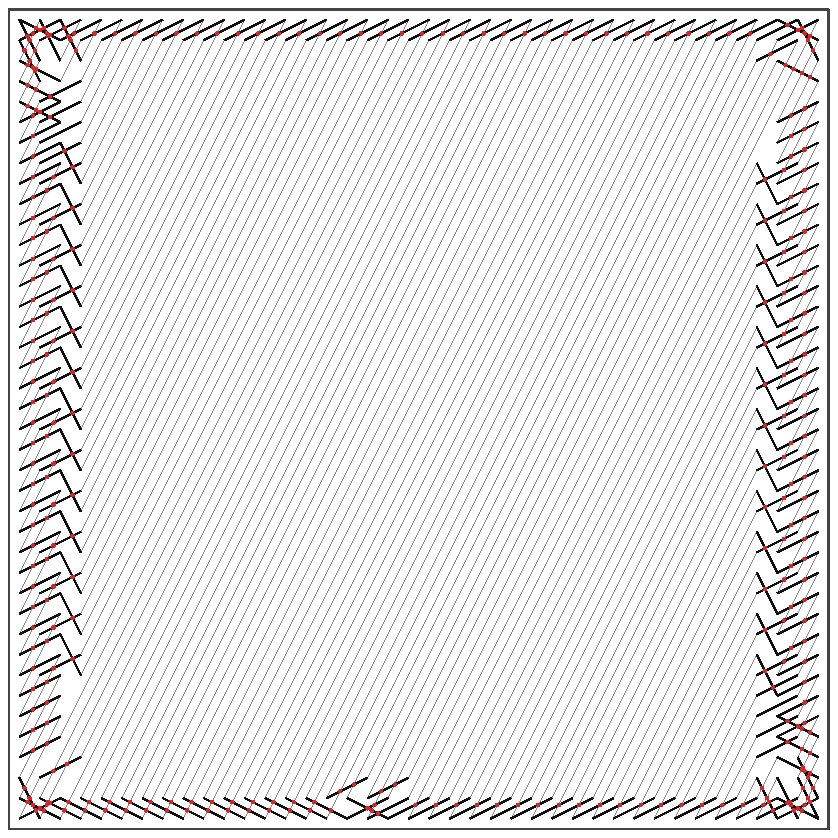
\includegraphics[width=0.72\textwidth]{fig_tour40.pdf}
\caption{The tour $T_{40}$. It has $313=7.5\cdot40+13$ crossings, marked by red dots; all of them are near the
walls. Grey: moves of the field. Black: the other moves.}
\label{fig:tour}
\end{figure}

\section{The field and the wall patterns}\label{sec:patterns}
The cells are the pairs $(x,y)$ with $0\le x,y<n$; $x$ is the column and $y$ the row, and the row $0$ is at the
bottom. A move joins two cells that differ by $(\pm1,\pm2)$ or $(\pm2,\pm1)$. Throughout, $n$ is even and $h=n/2$.

\subsection*{The field}
A \emph{field move} joins $(x,y)$ and $(x+1,y+2)$. Field moves are parallel, so no two of them cross. The cells
$(x,y)$ with $2x-y=k$ form the \emph{line}~$k$; a field move joins two consecutive cells of a line. The two field
moves at a cell $(x,y)$ are the moves to $(x+1,y+2)$ and to $(x-1,y-2)$.

\subsection*{The patterns at the top and at the bottom}
\begin{itemize}
\item Pattern $\mathsf A$ at the top wall consists of the moves $(x,n-2)\,\text{--}\,(x+2,n-1)$.
\item Pattern $\mathsf A$ at the bottom wall consists of the moves $(x,0)\,\text{--}\,(x+2,1)$.
\item Pattern $\mathsf B$ at the bottom wall consists of the moves $(x,0)\,\text{--}\,(x-2,1)$.
\end{itemize}
In each case a cell of the two outer rows has one move of the pattern and the field move that leads away from the
wall (Figure~\ref{fig:patterns}).

\subsection*{The patterns at the left and at the right}
The pattern at the left wall has period $2$ in $y$. It consists of the moves
\begin{align*}
&(0,y)\,\text{--}\,(1,y+2),\quad (0,y)\,\text{--}\,(2,y+1),\quad (3,y)\,\text{--}\,(4,y+2) &&\text{for all } y,\\
&(1,y)\,\text{--}\,(2,y+2) &&\text{for even } y,\\
&(1,y)\,\text{--}\,(3,y+1),\quad (3,y)\,\text{--}\,(2,y+2) &&\text{for odd } y.
\end{align*}
Every cell of the columns $0,\dots,3$ lies on exactly two of these moves, and a cell of the column $4$ on one; its
other move, and both moves of a cell of the column $5$, are field moves. The pattern at the right wall is the image
of the pattern at the left wall under a half turn of the board that maps even rows to odd rows. With $R_j=n-1-j$ it
consists of the moves
\begin{align*}
&(R_0,y)\,\text{--}\,(R_1,y-2),\quad (R_0,y)\,\text{--}\,(R_2,y-1),\quad (R_3,y)\,\text{--}\,(R_4,y-2) &&\text{for all } y,\\
&(R_1,y)\,\text{--}\,(R_3,y-1),\quad (R_2,y)\,\text{--}\,(R_3,y+2) &&\text{for even } y,\\
&(R_1,y)\,\text{--}\,(R_2,y-2) &&\text{for odd } y.
\end{align*}

\begin{figure}[t]
\centering
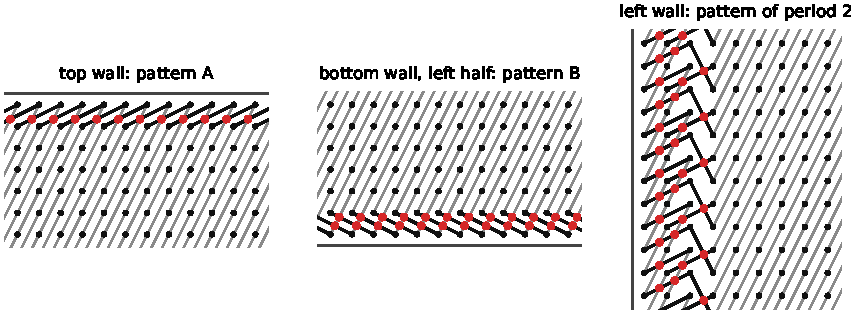
\includegraphics[width=\textwidth]{fig_patterns.pdf}
\caption{The patterns $\mathsf A$ (top wall), $\mathsf B$ (bottom wall) and the pattern at the left wall, each on
top of the field. Red dots mark the crossings: one per column, two per column, and five per two rows.}
\label{fig:patterns}
\end{figure}

\begin{lemma}\label{lem:cross}
Where a pattern is surrounded by itself and by the field, its crossings are as follows.
\begin{itemize}
\item[(a)] The move $(x,n-2)\,\text{--}\,(x+2,n-1)$ of $\mathsf A$ at the top crosses the field move
$(x,n-3)\,\text{--}\,(x+1,n-1)$ and no other move. The move $(x,0)\,\text{--}\,(x+2,1)$ of $\mathsf A$ at the bottom
crosses the field move $(x+1,0)\,\text{--}\,(x+2,2)$ and no other move.
\item[(b)] The move $(x,0)\,\text{--}\,(x-2,1)$ of $\mathsf B$ crosses the field moves $(x-2,0)\,\text{--}\,(x-1,2)$
and $(x-1,0)\,\text{--}\,(x,2)$ and no other move.
\item[(c)] The pattern at the left wall has $5$ crossings in every two rows, and so has the pattern at the right
wall.
\end{itemize}
So the patterns have $1$, $1$, $2$ crossings per column and $2.5$ crossings per row.
\end{lemma}
\begin{proof}
Two moves can cross only if their cells are within three rows and columns of each other, so each statement is a
finite check; the moves of one pattern are translates of each other, and for (c) one period suffices. In (c) the
five crossing pairs with lowest cell in the rows $0$ and $1$ are, for the left wall,
$\{(0,0)\text{--}(2,1),\ (1,0)\text{--}(2,2)\}$, $\{(1,0)\text{--}(2,2),\ (1,1)\text{--}(3,2)\}$,
$\{(1,1)\text{--}(3,2),\ (2,3)\text{--}(3,1)\}$, $\{(0,2)\text{--}(2,3),\ (0,1)\text{--}(1,3)\}$ and
$\{(0,0)\text{--}(1,2),\ (0,1)\text{--}(2,2)\}$. The program of Section~\ref{sec:files} counts all crossings of all
tours without using this lemma.
\end{proof}

\section{The tours}\label{sec:tours}
Let $n\ge30$ be even. The tour $T_n$ is defined by giving the two moves of every cell (Figures~\ref{fig:tour}
and~\ref{fig:patches}).
\begin{itemize}
\item[(i)] \emph{The field.} The cells $(x,y)$ with $6\le x\le n-7$ and $3\le y\le n-4$; the cells $(x,n-3)$ with
$4\le x\le n-5$; and the cells $(x,2)$ with $2\le x\le h-4$ or $h\le x\le n-5$. Each has its two field moves.
\item[(ii)] \emph{Top wall.} The cells $(x,n-2)$ with $3\le x\le n-6$ and the cells $(x,n-1)$ with
$5\le x\le n-4$. Each has its move of pattern $\mathsf A$ and the field move that leads down.
\item[(iii)] \emph{Bottom wall.} The cells $(x,0)$ with $5\le x\le h-5$ and $(x,1)$ with $3\le x\le h-7$ have their
move of pattern $\mathsf B$; the cells $(x,0)$ with $h-1\le x\le n-6$ and $(x,1)$ with $h+1\le x\le n-4$ have their
move of pattern $\mathsf A$; each has also the field move that leads up.
\item[(iv)] \emph{Left and right walls.} The cells of the columns $0,\dots,5$ and $n-6,\dots,n-1$ in the rows
$8\le y\le n-9$. Each has the moves that the pattern at the left wall, or at the right wall, gives it.
\item[(v)] \emph{Patches.} The cells that are not named in (i)--(iv). There are $179$ of them: $40$ near the bottom
left corner, $42$ near each of the other corners, and $13$ near the middle of the bottom wall, namely $(x,0)$ for
$h-4\le x\le h-2$, $(x,1)$ for $h-6\le x\le h$ and $(x,2)$ for $h-3\le x\le h-1$. Such a cell has the moves of the
cell of the board of side $40$ that lies at the same place relative to the nearest corner, or relative to the
column $h$ for the $13$ cells, in the tour $T_{40}$ that is given in the file \texttt{tour40.txt}.
\end{itemize}
The tour $T_{40}$ of the file satisfies (i)--(iv), so the definition is consistent for $n=40$.

\begin{figure}[t]
\centering
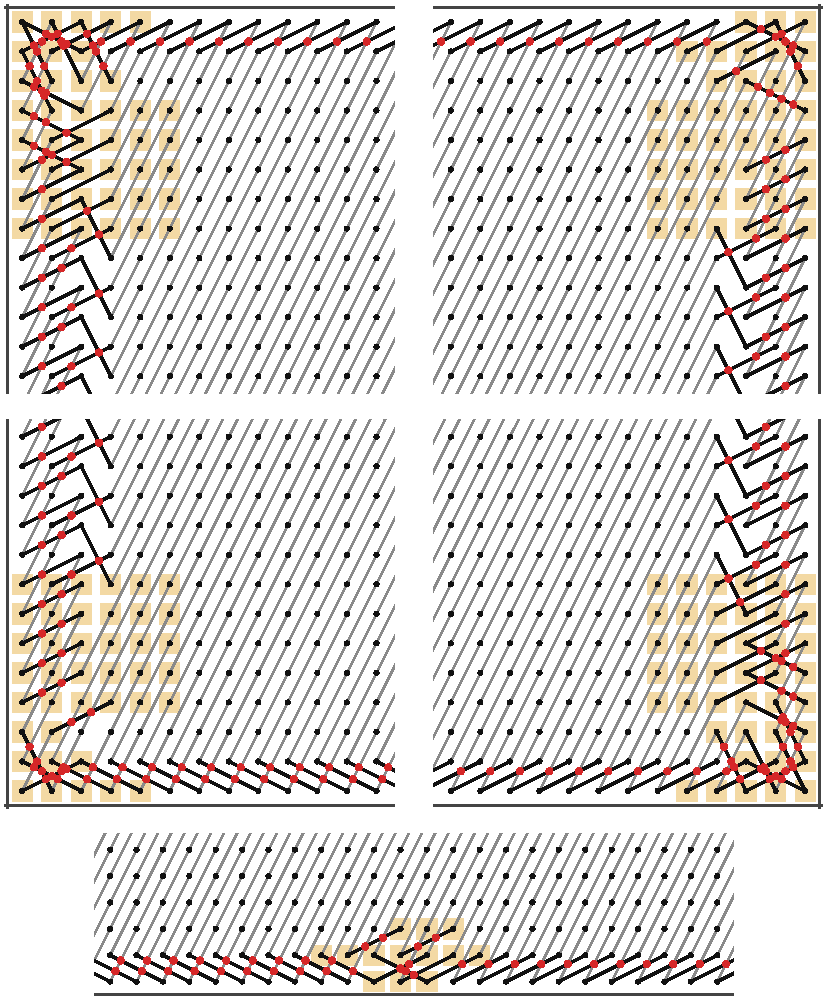
\includegraphics[width=0.78\textwidth]{fig_patches.pdf}
\caption{The four corners of $T_{40}$ and the middle of its bottom wall. The cells of the patches are shaded.
Everything else is the field and the four wall patterns.}
\label{fig:patches}
\end{figure}

\begin{proposition}\label{prop:cover}
For every even $n\ge30$, the moves of $T_n$ are well defined: every move that is listed at a cell is also listed at
its other cell.
\end{proposition}
\begin{proof}
A move joins cells at distance at most $2$ in each coordinate. The regions (i)--(iv) end at fixed distances from the
corners and from the column $h$, and the patterns have period $1$ or $2$. So for $n\ge40$ the cells within distance
$2$ of a patch form the same configuration as in $T_{40}$ or in $T_{42}$, up to a translation by even numbers, and
every other cell and its neighbours form a piece of the field and the patterns, which fit together as described in
Section~\ref{sec:patterns}. The program checks the statement directly for $30\le n\le500$, by building the tour and
testing that the listed moves give every cell exactly two.
\end{proof}

\section{Proof of the theorem}\label{sec:proof}
\subsection*{The number of crossings}
\begin{lemma}\label{lem:count}
$T_{n+2}$ has $15$ crossings more than $T_n$, for every even $n\ge30$.
\end{lemma}
\begin{proof}
For $n\le52$ the program counts. Let $n\ge54$. Field moves do not cross each other, and every other move of $T_n$
joins two cells within the three outer rows or the four outer columns. Two moves that cross have all their cells
within three rows and columns of each other. So a crossing lies either near a patch, where $T_n$ and $T_{n+2}$
look the same, or inside a stretch of one pattern, which is longer than $10$ columns or rows. From $T_n$ to
$T_{n+2}$ the top wall gets two more columns of $\mathsf A$, the bottom wall one more column of $\mathsf B$ and one
of $\mathsf A$, and the left and right walls two more rows each. By Lemma~\ref{lem:cross} this adds $2+2+1+5+5=15$
crossings.
\end{proof}
Since $T_{30}$ has $238$ crossings, $T_n$ has $7.5\,n+13$ crossings.

\subsection*{Strands and joins}
In $T_n$ call the cells $(x,y)$ with $6\le x\le n-7$ and $3\le y\le n-4$ \emph{inner} cells; they have field
moves. The inner cells of a line $k$ are consecutive on it; they form the \emph{strand} $k$. It has a lower end
and an upper end, which we write $(k,\lo)$ and $(k,\hi)$. There are $3n-32$ strands, with $16-n\le k\le 2n-17$.
Following $T_n$ from an end of a strand through cells that are not inner, one arrives at an end of another strand;
we say that the two ends are \emph{joined}, and we call the cells in between the path of the join. So $T_n$ is a
single closed tour if and only if the strands, with these joins, form a single cycle and every cell that is not
inner lies on the path of a join.

\begin{lemma}\label{lem:joins}
Where the patterns apply, the joins are as follows, for even $k$.
\begin{itemize}
\item[(a)] At the top wall $(k,\hi)$ is joined to $(k+3,\hi)$.
\item[(b)] At the bottom wall, pattern $\mathsf B$ joins $(k,\lo)$ to $(k-5,\lo)$, and pattern $\mathsf A$ joins
$(k,\lo)$ to $(k+3,\lo)$.
\item[(c)] At the left wall $(k,\lo)$ is joined to $(k+7,\lo)$, and at the right wall $(k,\hi)$ to $(k+7,\hi)$.
\end{itemize}
In (c) the path of the join has twelve cells, and these paths together pass through every cell of the six outer
columns once.
\end{lemma}
\begin{proof}
(a) The line $k$ with $k$ even meets the row $n-2$ in the cell $(x,n-2)$ with $2x=k+n-2$, and the tour continues
from there to $(x+2,n-1)$, the last cell of the line $2(x+2)-(n-1)=k+3$, and then down this line.
(b) The cell $(x,0)$ is the first cell of the line $2x$; pattern $\mathsf B$ joins it to $(x-2,1)$, the first cell
of the line $2x-5$, and pattern $\mathsf A$ joins it to $(x+2,1)$, the first cell of the line $2x+3$.
(c) At the left wall the line $k$ arrives from the right at the cell $(5,10-k)$. For even $k$ the tour continues
\begin{multline*}
(5,10-k),\ (4,8-k),\ (3,6-k),\ (1,5-k),\ (0,3-k),\ (2,4-k),\\ (1,2-k),\ (0,-k),\ (2,1-k),\ (3,-1-k),\ (4,1-k),\ (5,3-k)
\end{multline*}
by the moves of the pattern, and $(5,3-k)$ lies on the line $k+7$. This path contains one cell in each of the
columns $0,\dots,5$ and each parity of the row, so the paths for the even $k$ contain every cell of these columns
once. The right wall is the image of the left wall under a half turn, which maps the line $k$ to the line $c-k$
with an odd constant $c$ and lower ends to upper ends.
\end{proof}

We say that a join \emph{follows a rule} if it is one of the pairs in Lemma~\ref{lem:joins}:
$(k,\hi)\,\text{--}\,(k+3,\hi)$, $(k,\lo)\,\text{--}\,(k-5,\lo)$, $(k,\lo)\,\text{--}\,(k+3,\lo)$,
$(k,\lo)\,\text{--}\,(k+7,\lo)$ or $(k,\hi)\,\text{--}\,(k+7,\hi)$ with $k$ even.

\begin{table}[t]
\centering
\small\setlength{\tabcolsep}{4pt}
\begin{tabular}{llr@{\quad\ }llr}
near & join & cells & near & join & cells\\ \hline
top left & $(17-n,\hi)$ -- $(21-n,\lo)$ & $15$ & bottom middle & $(n-7,\lo)$ -- $(n-4,\lo)$ & $2$\\
top left & $(17-n,\lo)$ -- $(19-n,\lo)$ & $57$ & top right & $(n-8,\hi)$ -- $(n+3,\hi)$ & $14$\\
bottom left & $(-6,\lo)$ -- $(0,\lo)$ & $15$ & top right & $(n-5,\hi)$ -- $(n-2,\hi)$ & $8$\\
bottom left & $(-4,\lo)$ -- $(4,\lo)$ & $15$ & top right & $(n-3,\hi)$ -- $(n+5,\hi)$ & $15$\\
bottom left & $(-2,\lo)$ -- $(2,\lo)$ & $13$ & bottom right & $(2n-22,\hi)$ -- $(2n-18,\lo)$ & $15$\\
bottom middle & $(n-13,\lo)$ -- $(n-5,\lo)$ & $3$ & bottom right & $(2n-20,\hi)$ -- $(2n-18,\hi)$ & $57$\\
bottom middle & $(n-11,\lo)$ -- $(n-8,\lo)$ & $2$ &&&\\
bottom middle & $(n-9,\lo)$ -- $(n-1,\lo)$ & $3$ &&&
\end{tabular}
\caption{The fourteen joins of $T_n$ that follow no rule, with the number of cells on their paths.}
\label{tab:exc}
\end{table}

\begin{lemma}\label{lem:exc}
Let $n\ge30$ be even. Every cell of $T_n$ that is not inner lies on the path of exactly one join. The joins are
the fourteen joins of Table~\ref{tab:exc} and, for even $k$, the joins
\begin{itemize}
\item $(k,\lo)\,\text{--}\,(k+7,\lo)$ (left rule) for $16-n\le k\le-8$;
\item $(k,\hi)\,\text{--}\,(k+3,\hi)$ (top rule) for $16-n\le k\le n-10$ and for $k=n-4$;
\item $(k,\lo)\,\text{--}\,(k-5,\lo)$ (rule $\mathsf B$) for $6\le k\le n-10$;
\item $(k,\lo)\,\text{--}\,(k+3,\lo)$ (rule $\mathsf A$) for $k=n-6$ and for $n-2\le k\le2n-20$;
\item $(k,\hi)\,\text{--}\,(k+7,\hi)$ (right rule) for $k=n-6$ and for $n\le k\le2n-24$.
\end{itemize}
\end{lemma}
These are $3n-32$ joins, and each of the $2(3n-32)$ ends of strands occurs in exactly one of them. To see this, here
are the ends of each kind with the join they lie in (T: Table~\ref{tab:exc}).
\begin{itemize}
\item Lower ends, $k$ even: $16-n,\dots,-8$ left; $-6,\dots,4$ T; $6,\dots,n-10$ $\mathsf B$; $n-8$ T; $n-6$ $\mathsf A$;
$n-4$ T; $n-2,\dots,2n-20$ $\mathsf A$; $2n-18$ T.
\item Upper ends, $k$ even: $16-n,\dots,n-10$ top; $n-8$ T; $n-6$ right; $n-4$ top; $n-2$ T; $n,\dots,2n-24$ right;
$2n-22$, $2n-20$, $2n-18$ T.
\item Lower ends, $k$ odd: $17-n$, $19-n$, $21-n$ T; $23-n,\dots,-1$ left; $1,\dots,n-15$ $\mathsf B$; $n-13$, $n-11$, $n-9$,
$n-7$, $n-5$ T; $n-3$ $\mathsf A$; $n-1$ T; $n+1,\dots,2n-17$ $\mathsf A$.
\item Upper ends, $k$ odd: $17-n$ T; $19-n,\dots,n-7$ top; $n-5$, $n-3$ T; $n-1$ top; $n+1$ right; $n+3$, $n+5$ T;
$n+7,\dots,2n-17$ right.
\end{itemize}

\begin{proof}
\emph{Ends and their paths.} The lower end of an even strand $k$ is the cell $(\frac{k+4}2,4)$ if $k\ge8$ and the cell
$(6,12-k)$ if $k\le8$; the upper end is $(\frac{k+n-4}2,n-4)$ if $k\le n-10$ and $(n-7,2n-14-k)$ if $k\ge n-10$. From such
an end the moves of the patterns lead along the path of Lemma~\ref{lem:joins} for the wall at which the end lies. By
(i)--(iv), these paths contain no cell of a patch exactly in the following cases, and then the join is that of
Lemma~\ref{lem:joins}: the left rule for $20-n\le k\le-10$, the top rule for $16-n\le k\le n-12$, rule $\mathsf B$ for
$14\le k\le n-10$, rule $\mathsf A$ for $n-2\le k\le 2n-20$ and the right rule for $n+2\le k\le 2n-28$, with paths of $12$,
$3$, $3$, $3$ and $12$ cells. Each of these joins contains one even end. The remaining $28$ even ends are the even ends of the
joins in (a) below.

\emph{Base cases and two facts.} For $30\le n\le54$ the program checks the lemma (\texttt{--joins}) and, for
$40\le n\le54$, two more facts.
\begin{itemize}
\item[(a)] Exactly $28$ joins have a path that contains a cell of a patch: the fourteen of Table~\ref{tab:exc}, with the
numbers of cells given there, and fourteen joins that follow a rule: the left rule for $k=16-n$, $18-n$, $-8$ ($12$ cells
each); the top rule for $k=n-10$ ($4$ cells) and $k=n-4$ ($10$ cells); rule $\mathsf B$ for $k=6$, $8$, $10$, $12$ ($8$,
$8$, $5$, $4$ cells); rule $\mathsf A$ for $k=n-6$ ($3$ cells); and the right rule for $k=n-6$, $n$, $2n-26$, $2n-24$
($12$ cells each).
\item[(b)] The path of each of these $28$ joins lies in one of five \emph{boxes}: the cells within $9$ columns of the left or
right wall and within $20$ rows of the top or bottom wall, which form one box at each corner, and the columns
$h-7,\dots,h+1$ of the rows $0$, $1$, $2$ (the middle box). Namely, a join of Table~\ref{tab:exc} lies in the box named in
its column ``near''; the left rule at $-8$ and rule $\mathsf B$ in the bottom left box; the left rule at $16-n$ and $18-n$ in
the top left box; rule $\mathsf A$ at $n-6$ in the middle box; the top rule and the right rule at $n-6$ and $n$ in the top
right box; and the right rule at $2n-26$ and $2n-24$ in the bottom right box.
\end{itemize}

\emph{Induction.} Let $n\ge56$ and suppose that the lemma, (a) and (b) hold for $n-2$. The boxes do not meet. The
conditions (i)--(v) on the cells of a box are stated relative to the nearest corner, or to the column $h$ for the middle
box, and the patterns have period $1$ or $2$. So each box of $T_n$, with the moves of its cells, is the translate of the
corresponding box of $T_{n-2}$ by $(0,0)$, $(0,2)$, $(2,2)$, $(2,0)$ or $(1,0)$, for the bottom left, top left, top right
and bottom right box and the middle box. A translation by $(a,b)$ maps the line $k$ to the line $k+2a-b$; so it adds $0$,
$-2$, $2$, $4$ and $2$ to the indices, and these are exactly the changes from $n-2$ to $n$ of the indices in (a) and in
Table~\ref{tab:exc} that belong to that box (for instance $17-(n-2)-2=17-n$ and $(n-2)-13+2=n-13$). Each cell of a patch of
$T_n$ is the translate of a cell of a patch of $T_{n-2}$, which lies on one of the $28$ paths of (a). That path stays in its
box, so its translate is a path of $T_n$, with the same number of cells, that joins the translated ends. So (a) and (b)
hold for $n$, and with the first paragraph we have all the joins of the statement.

\emph{Every cell lies on a path.} Paths of different joins are disjoint, since every cell has two moves. The paths of
Table~\ref{tab:exc} have $234$ cells, and those of the fourteen joins in (a) that follow a rule have $126$. The other
$n-28$ joins at the left and right walls have $12$ cells each, and the other $2n-32$ joins at the top and bottom walls
have $3$. In all this is $234+126+12(n-28)+3(2n-32)=18n-72$, which is the number of cells that are not inner. So each of
them lies on exactly one path.
\end{proof}

\subsection*{Passes}
A \emph{pass} is a maximal sequence of strands in which consecutive strands are joined by joins that follow a rule. So
the first and the last strand of a pass have an end in a join of Table~\ref{tab:exc}, and the cycles formed by the strands
and the joins consist of passes, which are joined to each other by the joins of Table~\ref{tab:exc}.

\begin{table}[t]
\centering
\footnotesize
\begin{tabular}{l@{\ \ }l}
$n\bmod 8$ & the fourteen passes, in the order of the tour\\ \hline
$0$ & $-6\to21-n$;\ \ $17-n$;\ \ $19-n\to-4$;\ \ $4\to n-9$;\ \ $n-1\to n-4$;\ \ $n-7\to-2$;\ \ $2\to n-11$;\\
 & $n-8$;\ \ $n+3\to2n-20$;\ \ $2n-18$;\ \ $2n-22\to n+5$;\ \ $n-3\to n-2$;\ \ $n-5$;\ \ $n-13\to0$\\[3pt]
$2$ & $-6\to19-n$;\ \ $17-n$;\ \ $21-n\to-4$;\ \ $4\to n-11$;\ \ $n-8$;\ \ $n+3\to2n-22$;\ \ $2n-18$;\\
 & $2n-20\to n+5$;\ \ $n-3\to n-2$;\ \ $n-5$;\ \ $n-13\to2$;\ \ $-2\to n-9$;\ \ $n-1\to n-4$;\ \ $n-7\to0$\\[3pt]
$4$ & $-6\to21-n$;\ \ $17-n$;\ \ $19-n\to-4$;\ \ $4\to n-13$;\ \ $n-5$;\ \ $n-2\to n-3$;\ \ $n+5\to2n-22$;\\
 & $2n-18$;\ \ $2n-20\to n+3$;\ \ $n-8$;\ \ $n-11\to-2$;\ \ $2\to n-7$;\ \ $n-4\to n-1$;\ \ $n-9\to0$\\[3pt]
$6$ & $-6\to19-n$;\ \ $17-n$;\ \ $21-n\to-4$;\ \ $4\to n-7$;\ \ $n-4\to n-1$;\ \ $n-9\to2$;\ \ $-2\to n-13$;\\
 & $n-5$;\ \ $n-2\to n-3$;\ \ $n+5\to2n-20$;\ \ $2n-18$;\ \ $2n-22\to n+3$;\ \ $n-8$;\ \ $n-11\to0$
\end{tabular}
\caption{The passes of $T_n$: first and last strand of each (a single index is a pass of one strand). Consecutive
passes, and the last and the first, are joined by joins of Table~\ref{tab:exc}.}
\label{tab:pass}
\end{table}

\begin{lemma}\label{lem:step}
Let $n\ge30$ be even. The strands of $T_n$ and their joins form a single cycle, which consists of the fourteen
passes of Table~\ref{tab:pass} in the order given there. Hence $T_n$ is a single closed tour.
\end{lemma}
\begin{proof}
We use only the list of joins in Lemma~\ref{lem:exc}; all indices below that are called $k$ are even.
\begin{itemize}
\item[(1)] For $16-n\le k\le-4$ the top rule joins $(k,\hi)$ and $(k+3,\hi)$, and for $20-n\le k\le-4$ the left rule joins
$(k+3,\lo)$ and $(k-4,\lo)$. So the strands $k$ and $k+3$ with $16-n\le k\le-4$ form passes $k,\ k+3,\ k-4,\ k-1,\ k-8,\dots$,
one for each class of $k$ modulo $4$. Each runs from $k_0\in\{-6,-4\}$ to the strand among $19-n$, $21-n$ that is congruent
to $k_0+3$ modulo $4$; the lower ends of these strands are in Table~\ref{tab:exc}.
\item[(2)] For $-2\le k\le n-10$ the top rule joins $(k,\hi)$ and $(k+3,\hi)$, and for $-2\le k\le n-18$ rule $\mathsf B$
joins $(k+3,\lo)$ and $(k+8,\lo)$. So the strands $k$ and $k+3$ with $-2\le k\le n-10$ form passes
$k,\ k+3,\ k+8,\ k+11,\dots$, one for each class of $k$ modulo $8$. Each runs from $k_0\in\{-2,0,2,4\}$ to the strand among
$n-13$, $n-11$, $n-9$, $n-7$ that is congruent to $k_0+3$ modulo $8$; the lower ends of these strands are in
Table~\ref{tab:exc}.
\item[(3)] For $n\le k\le 2n-20$ rule $\mathsf A$ joins $(k,\lo)$ and $(k+3,\lo)$, and for $n\le k\le 2n-24$ the right rule
joins $(k,\hi)$ and $(k+7,\hi)$. So the strands $k$ and $k+3$ with $n\le k\le 2n-20$ form passes
$k+3,\ k,\ k+7,\ k+4,\ k+11,\dots$, one for each class of $k$ modulo $4$. Each runs between the strand among $n+3$, $n+5$
and the strand among $2n-22$, $2n-20$ that belong to its class; the upper ends of these strands are in Table~\ref{tab:exc}.
\item[(4)] The ten other strands form six passes: $17-n$, $n-8$, $n-5$ and $2n-18$ alone; $n-4,\ n-1$ (top rule at $n-4$);
and $n-2,\ n+1,\ n-6,\ n-3$ (rule $\mathsf A$ at $n-2$, the right rule at $n-6$, rule $\mathsf A$ at $n-6$).
\end{itemize}
Together these fourteen passes contain $(n-18)+(n-6)+(n-18)+10=3n-32$ strands, that is, every strand once. Which strand
ends a pass in (1)--(3) depends only on the class of $n$ modulo $8$. In each of the four classes, following the joins of
Table~\ref{tab:exc} from the end of one pass to the next gives the cyclic order of Table~\ref{tab:pass}, a check of fourteen
steps; in particular all strands lie on one cycle. (The program repeats this from the list of Lemma~\ref{lem:exc} for
$30\le n\le3000$, \texttt{--arith}, and on the tours themselves for $30\le n\le300$, \texttt{--joins}.) By
Lemma~\ref{lem:exc} every cell that is not inner lies on exactly one join, so $T_n$ is a single closed tour.
\end{proof}

\begin{proof}[Proof of Theorem~\ref{thm:main}]
By Proposition~\ref{prop:cover} and Lemma~\ref{lem:step}, $T_n$ is a closed knight's tour of the $n\times n$ board
for every even $n\ge30$, and by Lemma~\ref{lem:count} it has $7.5\,n+13$ crossings.
\end{proof}

For $n=40$ the fourteen passes have $10$, $1$, $12$, $8$, $2$, $10$, $8$, $1$, $12$, $1$, $10$, $4$, $1$ and $8$
strands, in the order of Table~\ref{tab:pass}.

\section{Remarks on the ingredients}\label{sec:remarks}
The tours were found with the CP-SAT solver of OR-Tools~\cite{ortools}: first small periodic problems for one wall
were solved to optimality, then the patches of a board in which everything else was prescribed. The following
statements are reports of such runs, for the sizes stated; they are not used in the proof of the theorem.

\begin{remark}[The top and bottom walls]
Consider a strip that is periodic along a wall, with the field below it, and ask for moves that give every cell two
moves and agree with the field at depth $4$ or more. For the periods $4$, $6$ and $8$ the solver finds that the
least number of crossings is one per column, that pattern $\mathsf A$ is the only pattern that attains it, and that
no pattern has more than one and fewer than two crossings per column. With two crossings per column there are
several, among them $\mathsf B$.
\end{remark}

\begin{remark}[Why the bottom wall is not all $\mathsf A$]
By Lemma~\ref{lem:joins}, $\mathsf A$ at the top and $\mathsf A$ at the bottom both join the strand $k$ to the strand
$k+3$. Two strands that run from the bottom wall to the top wall would then be joined at both ends, and they would
form a closed cycle. This is why the left half of the bottom wall carries $\mathsf B$: the strands that begin there
end at the right half of the top wall. If the previous remark holds for all periods and depths, one of two walls
that are joined by strands always costs at least two crossings per column.
\end{remark}

\begin{remark}[The left and right walls]
At these walls the field arrives at a small angle, with one strand per row. For the periods $4$, $6$ and $8$ the
solver finds that the least numbers of crossings per period are $10$, $11$ and $16$. The pattern used here has $10$
crossings per four rows; it has period $2$. The patterns with $16$ crossings per eight rows and those with $11$
per six rows cannot be combined with $\mathsf A$ at the other end of the strands (pairs of strands would close up,
or the number of passes would be odd), only with $\mathsf B$. With period $8$ this gives $7.5\,n$ again. With
period $6$ it is a little better: put $\mathsf B$ on the left half of the top wall and on the whole bottom wall,
$\mathsf A$ on the right half of the top wall, and a pattern of period $6$ at the left and right walls; this costs
$1.5\,n+2n+\frac{11}{3}n=\frac{43}{6}n$. The solver completes such a tour of side $48$ with $368$ crossings (file
\texttt{variant48.txt}), and inserting periods into it gives closed tours with $\frac{43}{6}n+24$ crossings for
$n=48,60,72,\dots$; the program checks them up to $n=600$ (\texttt{--variant}). We have not worked out the other
classes of $n$ modulo $12$, nor a proof for all $n$ in this class, so Theorem~\ref{thm:main} is stated with the
constant $7.5$.
\end{remark}

\begin{remark}[Small boards]
For $n=6$ the least number of crossings is $52$ (the solver; also an enumeration of all $9862$ closed tours). For
$n=8$ it is $69$ according to the census reported in the answer to exercise 160 of~\cite{knuth}; the solver finds a
tour with $69$ crossings and proves only that at least $65$ are needed. For $n=10$ and $n=12$ it finds tours with
$83$ and $100$ crossings and proves the bounds $76$ and $85$.
\end{remark}

\begin{question}
Let $c(n)$ be the least number of crossings of a closed $n\times n$ knight's tour. What are
$\liminf c(n)/n$ and $\limsup c(n)/n$? They are at least $4$~\cite{besa} and at most $7.5$; the variant above
suggests at most $43/6$.
\end{question}
One may try to meet all four walls at a steep angle, by dividing the board into eight sectors with different fields;
the moves of two such fields that meet along a diagonal or along an axis of the board need not cross. Then pattern
$\mathsf A$ and its mirror images would cost only one crossing per unit of wall. We could not complete the corners
of such an arrangement, not even to a cycle cover, and there is a reason. Take a square region at a corner with an
even side. It has equally many cells of the two colours of the chessboard, and every move joins cells of different
colours; so the moves that lead from the region to the outside must end, inside, on equally many cells of each
colour. In this arrangement, with patterns $\mathsf A$ or $\mathsf B$ on the two walls, they end on two more cells of
one colour than of the other. Moving the line along which two fields meet, or replacing it by three parallel lines
within six cells of the diagonal, changes this surplus to $1$, $2$, $4$ or $5$, never to $0$. We do not know whether
another arrangement does better.

\section{Verification and files}\label{sec:files}
The program \texttt{crossing\_tours.py} uses only the Python standard library.
\begin{itemize}
\item It builds $T_n$ from the description (i)--(v) and the file \texttt{tour40.txt}. For a given tour it checks
that every move is a knight's move, that every cell has two moves, and that the moves form one cycle through all
$n^2$ cells; and it counts the crossings by testing pairs of moves in exact integer arithmetic.
\item \texttt{--range 30 500}: every $T_n$ in this range is a closed tour with $7.5\,n+13$ crossings. The same was
checked for $n=1000$, $1002$ and $2000$.
\item \texttt{--joins 30 300}: for every $n$ in this range the joins of $T_n$ are exactly those of
Lemma~\ref{lem:exc}, every cell that is not inner lies on one join, the passes are those of Table~\ref{tab:pass}, and
(for $n\ge40$) the facts (a) and (b) in the proof of Lemma~\ref{lem:exc} hold, with the numbers of cells and the boxes
stated there.
\item \texttt{--arith 30 3000}: the $3n-32$ joins of Lemma~\ref{lem:exc}, taken as pairs of integers, form a single cycle
through all strands, with the passes of Table~\ref{tab:pass}. (A referee ran it up to $n=10000$.)
\item \texttt{--patterns 40 500}: a second construction, which inserts periods into $T_{40}$ or $T_{42}$, gives
the same tours.
\item \texttt{--steps 40 300}: the cyclic sequence of strands of $T_{n+8}$ is that of $T_n$ with $24$ strands
inserted.
\end{itemize}
The search programs (\texttt{template.py} and the programs for one wall) need OR-Tools.

Two separate AI agents refereed the paper. The first, given only an earlier version of this text and the tour files,
rebuilt $T_n$ from the description with programs of its own for every even $n$ from $40$ to $700$ and for six larger $n$
up to $2002$, and found the same tours, move for move. It found no error in the construction; it asked for the two tables
and for a proof in place of a sketch, and it observed that one set of patches serves for all $n\ge30$. The second checked
Sections~\ref{sec:tours} and~\ref{sec:proof} against the program; the list of ends after Lemma~\ref{lem:exc}, the counting
argument at the end of its proof and the direct proof of Lemma~\ref{lem:step} follow its suggestions.

\subsection*{Use of AI}
The search programs, the construction, the proofs and this manuscript were produced with Claude (Anthropic) under
the author's direction. The author is responsible for the content.

\begin{thebibliography}{9}
\bibitem{besa} J.~J.~Besa, T.~Johnson, N.~Mamano, M.~C.~Osegueda and P.~Williams, Taming the knight's tour:
minimizing turns and crossings, \emph{Theoretical Computer Science} 902 (2022), 1--20; arXiv:1904.02824.
\bibitem{knuth} D.~E.~Knuth, \emph{The Art of Computer Programming}, Volume 4, Pre-Fascicle 8A: \emph{Hamiltonian
Paths and Cycles}, draft of 8 May 2026, exercises 7.2.2.4--160 and 161 and their answers.
\url{https://www-cs-faculty.stanford.edu/~knuth/fasc8a.ps.gz}
\bibitem{ortools} L.~Perron and F.~Didier, CP-SAT, Google OR-Tools.
\url{https://developers.google.com/optimization/cp/cp_solver}
\end{thebibliography}
\end{document}
